% einleitung.tex
\chapter{Einleitung}
\section{Motivation und Hintergrund}
Im Laufe der Zeit ist deutlich geworden, dass eingebettete Systeme eine zunehmend wichtigere Rolle im alltäglichen Leben des Menschen spielen. Nahezu jedes elektrische Gerät enthält heutzutage eingebettete Rechnerhardware und viele lassen sich aus der Entfernung steuern. Es hat sich der Begriff Internet der Dinge (IoT) geprägt.

\begin{figure}[h]
	\centering
	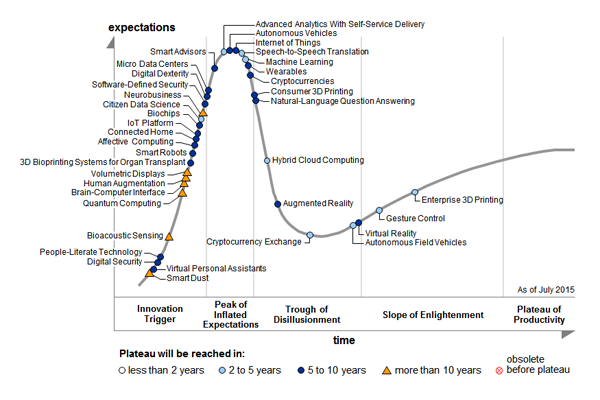
\includegraphics{bilder/hype}
	\caption{Der Hype Zyklus \cite{hype}}
	\label{fig:hype}
\end{figure}

Aus einer wissenschaftlichen Perspektive befindet sich das Internet der Dinge gerade auf dem Gipfel der überzogenen Erwartungen (siehe Abbildung \ref{fig:hype}). Auch der Autor dieser Arbeit ist davon nicht un­be­trof­fen.

Bevor das „Plateau der Produktivität“ jedoch erreicht wird, muss noch viel geforscht werden. Es gibt Fragen zu beantworten, welche die Themen Architektur und Abhängigkeiten, Big Data, Robustheit, Offenheit, Sicherheit und weitere betreffen. Auch das Problem der mangelnden Standardisierung wird immer wieder aufgegriffen.\\

Ein aktuelles und sich gerade stark weiterentwickelndes Gebiet des Internets der Dinge ist Smart Home. Darunter versteht man den Einsatz von Sensoren und Aktoren zur Automatisierung des Verhaltens der intelligenten Geräte im Hause des Endnutzers. Die dadurch gewonnenen Komfort, Sicherheit und Flexibilität bieten eine Unterstützung für den Nutzer, die schwierig zu überschätzen ist. Besonders in dem Gesundheitspflege Bereich kommt Smart Home immer wieder zum Einsatz.\\

Das Internet hat sich über wenige Jahrzehnte von einer neuartigen Idee zu einem der Grundpfeiler der Welt entwickelt. Die Anzahl der existierenden Webservices ist nicht mehr überschaubar. 
Menschen nutzen eine zunehmend steigende Anzahl von Diensten täglich, oftmals in sich ständig wiederholenden Szenarien. 
Diese Szenarien zu automatisieren versprechen webbasierte Task Automation Services (TAS). Unter TAS versteht man Dienste, die es dem Nutzer ermöglichen Regeln für die Interaktionen zwischen unterschiedlichen Webservices zu definieren. Daraufhin werden diese spezifizierten Interaktionen von dem TAS übernommen.\\

Webbasierte Task Automation Services sind bis dato völlig unabhängig von Smart Home Lösungen. Gleichzeitig realisieren sie dieselben Kernideen auf eine vergleichbare Weise, nur in einem anderen Umfeld. Dennoch wurden bisher keine Versuche unternommen, diese unterschiedlichen Ansätze in einem gemeinsamen Kontext zu verschmelzen. Dies ist der Punkt, an dem diese Arbeit ansetzen soll.


\section{Ziele der Arbeit}
Ziel dieser Arbeit ist es die Welten von Smart Home und webbasierten Task Automation Services zusammen zu bringen. Es soll ein Demonstrator entwickelt werden, der die  Funktionalitäten beider Ansätze kombiniert und in einem gemeinsamen Kontext anbietet. Es sollen die Stärken der beiden Technologien hervorgehoben und ihre Schwächen durch die Kombination reduziert werden.

Konkreter sind die Ziele in Sektion \ref{sec:ziele} erläutert.


\section{Aufbau der Arbeit}
Nach der Einleitung wird der aktuelle Stand der Forschung bezüglich \textit{Internet der Dinge}, \textit{SmartHome} und \textit{Task Automation Services} vorgestellt und die Ziele der Arbeit daraus abgeleitet. Daraufhin wird in Kapitel 3 das Framework Eclipse SmartHome (ESH) vorgestellt. In Kapitel 4 wird konkret betrachtet, wie die Funktionalitäten eines Task Automation Services in ESH integriert werden können.

Im folgenden Kapitel 5 wird die Implementierung des Entwurfs mit Hilfe von entsprechenden
Diagrammen vorgestellt. Der Quell-Code ist auf der mit der Arbeit mitgelieferten
CD einsehbar. Danach wird in Abschnitt 6 die Implementierung evaluiert. Schließlich folgt
noch eine kurze Zusammenfassung der geleisteten Arbeit und ein Ausblick auf mögliche
Weiterentwicklungen in Kapitel 7.

